%%%%%%%%%%%%%%%%%%%%%%% PREAMBLE %%%%%%%%%%%%%%%%%%%%%%%%
\documentclass[../../Root.tex]{subfiles}
\begin{document}
%%%%%%%%%%%%%%%%%%%%%%% DOCUMENT %%%%%%%%%%%%%%%%%%%%%%%%
\chapter{Demo: Proofs, Margins, and Figures}

This section demonstrates how to use various features of the template.

\subsection{Subproofs with \texttt{\textbackslash spf}}

Here is a theorem that requires multiple subproofs:

\thm[thm:demo]{Sum of First $n$ Integers}{
For any positive integer $n$, we have
\[
1 + 2 + 3 + \cdots + n = \frac{n(n+1)}{2}.
\]
}

\begin{proof}
We prove this by strong induction on $n$.

\spf{Base Case ($n=1$)}{
When $n = 1$, the left side is just $1$, and the right side is $\frac{1 \cdot 2}{2} = 1$. Thus the formula holds for $n = 1$.
}

\spf{Inductive Step}{
Assume the formula holds for some $k \geq 1$. We show it holds for $k+1$.

By the inductive hypothesis:
\[
1 + 2 + \cdots + k = \frac{k(k+1)}{2}
\]

Adding $(k+1)$ to both sides:
\[
1 + 2 + \cdots + k + (k+1) = \frac{k(k+1)}{2} + (k+1) = \frac{k(k+1) + 2(k+1)}{2} = \frac{(k+1)(k+2)}{2}
\]

This is exactly the formula with $n = k+1$.
}

By induction, the formula holds for all positive integers $n$.
\end{proof}

\subsection{Margin Comments}

You can add comments in the margin using tufte-book's built-in commands:\marginnote{This is a margin note created with \texttt{\textbackslash marginnote\{...\}}. It appears in the right margin alongside the text.}

The main commands are:
\begin{itemize}
\item \texttt{\textbackslash marginnote\{text\}} -- Simple margin note (unnumbered)\marginnote{This is an unnumbered margin note.}
\item \texttt{\textbackslash sidenote\{text\}} -- Tufte's sidenote (numbered like footnotes)\sidenote{This is a sidenote. It's numbered and works like a footnote but appears in the margin.}
\item \texttt{\textbackslash footnote\{text\}} -- Standard footnote (also goes to margin in tufte)\footnote{This is a standard numbered footnote.}
\end{itemize}

You can also use symbolic footnotes for specific notes:
{\footnotesymbolstrue
\footnote{This is a symbolic footnote (dagger) using the custom \texttt{footnotesymbolstrue} switch.}
\footnote{This is another symbolic footnote (double dagger).}
}
And back to numbered:
\footnote{This is a numbered footnote again.}

\subsection{Figures in the Margin}

Tufte-book provides special environments for margin figures:

\begin{marginfigure}
\centering
\begin{tikzpicture}[scale=0.8]
\draw[->] (-0.5,0) -- (3,0) node[right] {$x$};
\draw[->] (0,-0.5) -- (0,2.5) node[above] {$y$};
\draw[thick,blue] (0,0) parabola (2,2);
\node at (1.5,1.5) {$y = x^2$};
\end{tikzpicture}
\caption{A simple parabola in the margin.}
\end{marginfigure}

To place a figure in the margin, use the \texttt{marginfigure} environment. The figure will automatically be placed in the margin area.

\begin{marginfigure}
\centering
\includegraphics[width=\linewidth]{images/test.png}
\caption{An image in the margin using \texttt{\textbackslash includegraphics}.}
\end{marginfigure}

You can also include external images in the margin using \texttt{\textbackslash includegraphics} inside a \texttt{marginfigure} environment.

\subsection{Tables in the Margin}

Similarly, you can place tables in the margin:

\begin{margintable}
\centering
\begin{tabular}{cc}
\toprule
$n$ & $n!$ \\
\midrule
1 & 1 \\
2 & 2 \\
3 & 6 \\
4 & 24 \\
5 & 120 \\
\bottomrule
\end{tabular}
\caption{First few factorials.}
\end{margintable}

Use the \texttt{margintable} environment for tables in the margin.
\newpage
\subsection{Full-Width Figures}

For larger figures that need more space, use \texttt{figure*}:

\begin{figure*}
\centering
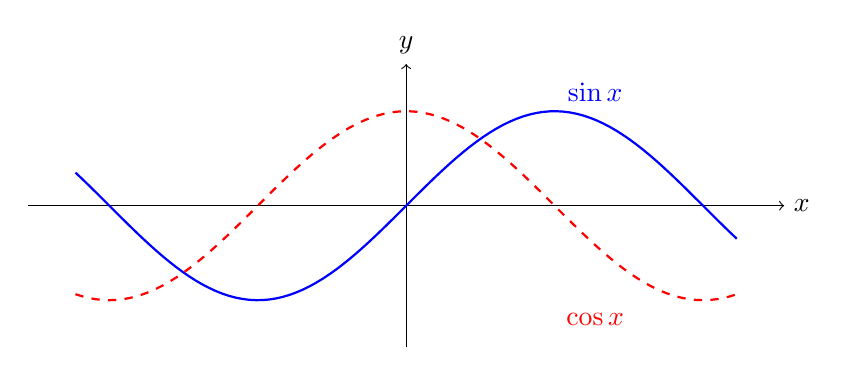
\begin{tikzpicture}[scale=1.2]
\draw[->] (-4,0) -- (4,0) node[right] {$x$};
\draw[->] (0,-1.5) -- (0,1.5) node[above] {$y$};
\draw[thick,blue,domain=-3.5:3.5,samples=100] plot (\x,{sin(\x r)});
\draw[thick,red,dashed,domain=-3.5:3.5,samples=100] plot (\x,{cos(\x r)});
\node[blue] at (2,1.2) {$\sin x$};
\node[red] at (2,-1.2) {$\cos x$};
\end{tikzpicture}
\caption{Sine and cosine functions spanning the full text width plus margin.}
\end{figure*}

\remm{
The \texttt{figure*} and \texttt{table*} environments span the full page width, including the margin area. These are useful for larger diagrams or tables.
}


\chapter{Example Chapter: Algebraic Foundations}

We begin by establishing the fundamental algebraic structures that underpin the study of Number Theory and Linear Algebra.\marginnote{We assume familiarity with the set of positive integers, denoted by $\mathbb{Z}^+ = \{1, 2, 3, \dots\}$.} While the rigorous construction of these numbers via the Peano axioms is foundational,\sidenote{Giuseppe Peano (1858--1932) formalized the axioms for natural numbers in 1889. His five axioms characterize $\mathbb{N}$ uniquely up to isomorphism.} we shall restrict our attention to their operational and order-theoretic properties.

\begin{marginfigure}
\centering
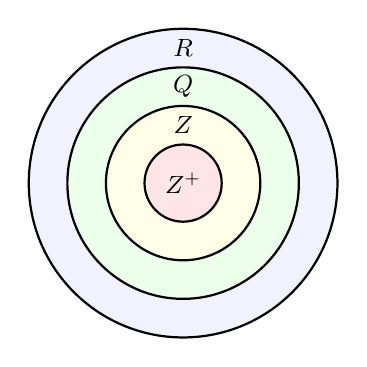
\begin{tikzpicture}[scale=0.7]
  % Number sets as nested circles
  \draw[thick, fill=blue!5] (0,0) circle (2.8cm);
  \draw[thick, fill=green!8] (0,0) circle (2.1cm);
  \draw[thick, fill=yellow!10] (0,0) circle (1.4cm);
  \draw[thick, fill=red!10] (0,0) circle (0.7cm);
  % Labels
  \node at (0,0) {\small $\mathbb{Z}^+$};
  \node at (0,1.05) {\small $\mathbb{Z}$};
  \node at (0,1.75) {\small $\mathbb{Q}$};
  \node at (0,2.45) {\small $\mathbb{R}$};
\end{tikzpicture}
\caption{The tower of number systems: each set is contained in the next.}
\end{marginfigure}

\section{The Integers}

Addition and multiplication are well-defined operations on $\mathbb{Z}^+$. For any $a, b \in \mathbb{Z}^+$, their sum $a+b$ and product $ab$ satisfy the following fundamental laws:\marginnote{These axioms form the basis of what algebraists call a \emph{commutative semiring}---a ring without additive inverses.}

\axiomm[ax:assoc_add]{Associativity of Addition}{For all $a, b, c \in \mathbb{Z}^+$, $(a+b)+c = a+(b+c)$.}
\axiomm[ax:comm_add]{Commutativity of Addition}{For all $a, b \in \mathbb{Z}^+$, $a+b = b+a$.}
\axiomm[ax:assoc_mult]{Associativity of Multiplication}{For all $a, b, c \in \mathbb{Z}^+$, $(ab)c = a(bc)$.}
\axiomm[ax:comm_mult]{Commutativity of Multiplication}{For all $a, b \in \mathbb{Z}^+$, $ab = ba$.}
\axiomm[ax:dist]{Distributivity}{For all $a, b, c \in \mathbb{Z}^+$, $a(b+c) = ab + ac$.}
\axiomm[ax:ident_mult]{Multiplicative Identity}{There exists an element $1 \in \mathbb{Z}^+$ such that for all $a \in \mathbb{Z}^+$, $a \cdot 1 = a$.}

The set $\mathbb{Z}^+$ is also endowed with a strict total ordering, denoted by $<$. For any $a, b \in \mathbb{Z}^+$, exactly one of the following holds:
\[ a < b, \quad a = b, \quad \text{or} \quad b < a. \]
This order respects the arithmetic operations:
\begin{enumerate}[nolistsep, label=(\roman*)]
    \item If $a < b$, then $a+c < b+c$ for any $c$.
    \item If $a < b$, then $ac < bc$ for any $c$.
    \item If $a < b$ and $b < c$, then $a < c$ (Transitivity).
\end{enumerate}

The structural essence of the positive integers is captured by the Induction Axiom.\sidenote{Induction formalizes the intuition that we can ``climb'' from $1$ to any positive integer by repeatedly adding $1$. This is sometimes called the \emph{domino principle}.}

\axiomm[ax:induction]{Induction Axiom}{Let $S \subseteq \mathbb{Z}^+$. If $S$ satisfies:
\begin{enumerate}[nolistsep, label=(\roman*)]
    \item $1 \in S$, and
    \item For any $k \in \mathbb{Z}^+$, $k \in S \implies k+1 \in S$,
\end{enumerate}
then $S = \mathbb{Z}^+$.}

\begin{marginfigure}
\centering
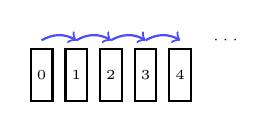
\begin{tikzpicture}[scale=0.55]
  % Dominoes
  \foreach \i in {0,1,2,3,4} {
    \draw[thick, fill=white] (\i*0.8,0) rectangle (\i*0.8+0.5,1.2);
    \node at (\i*0.8+0.25,0.6) {\tiny $\i$};
  }
  % Arrow showing the cascade
  \draw[->, thick, blue!70] (0.25,1.4) to[bend left=30] (1.05,1.4);
  \draw[->, thick, blue!70] (1.05,1.4) to[bend left=30] (1.85,1.4);
  \draw[->, thick, blue!70] (1.85,1.4) to[bend left=30] (2.65,1.4);
  \draw[->, thick, blue!70] (2.65,1.4) to[bend left=30] (3.45,1.4);
  \node at (4.5,1.4) {\tiny $\cdots$};
\end{tikzpicture}
\caption{The domino metaphor: if the first falls and each knocks down the next, all fall.}
\end{marginfigure}

This axiom provides the basis for the First Principle of Mathematical Induction.

\thm[thm:induction_1]{First Principle of Mathematical Induction}{Let $P(n)$ be a proposition regarding positive integers. If:
\begin{enumerate}[nolistsep, label=(\roman*)]
    \item $P(1)$ is true, and
    \item $P(k) \implies P(k+1)$ for any $k \in \mathbb{Z}^+$,
\end{enumerate}
then $P(n)$ is true for all $n \in \mathbb{Z}^+$.}

An equivalent and equally powerful property of $\mathbb{Z}^+$ is the existence of minimal elements in non-empty subsets.\footnote{The equivalence of induction and well-ordering is a deep result. In fact, in set theory, one often \emph{defines} the natural numbers as the smallest inductive set.}

\thm[thm:least_number]{Least Number Principle}{Let $S$ be a non-empty subset of $\mathbb{Z}^+$. Then there exists $m \in S$ such that for all $x \in S$, $m \le x$. We call $m$ the least element of $S$.}\marginnote{Also known as the \emph{Well-Ordering Principle}. This property fails spectacularly for $\mathbb{Q}$ and $\mathbb{R}$---consider the set $\{x \in \mathbb{Q} : x > 0\}$, which has no least element.}

Conversely, if a set is bounded from above, it possesses a maximal element.

\thm[thm:greatest_number]{Greatest Number Principle}{Let $S \subseteq \mathbb{Z}^+$ be non-empty. If $S$ has an upper bound (i.e., there exists $M \in \mathbb{Z}^+$ such that $x \le M$ for all $x \in S$), then there exists $g \in S$ such that for all $x \in S$, $x \le g$.}

The \nameref{thm:least_number} allows us to establish the Second Principle of Mathematical Induction (often called Strong Induction), which is frequently more useful when the recursive step depends on multiple preceding terms.\sidenote{Strong induction is essential for proving the Fundamental Theorem of Arithmetic: every integer $n > 1$ factors uniquely into primes. The proof requires knowing that \emph{all} smaller numbers factor, not just the predecessor.}

\thm[thm:strong_induction]{Second Principle of Mathematical Induction}{Let $P(n)$ be a proposition regarding positive integers. If:
\begin{enumerate}[nolistsep, label=(\roman*)]
    \item $P(1)$ is true, and
    \item For any $k \in \mathbb{Z}^+$, if $P(j)$ holds for all $1 \le j \le k$, then $P(k+1)$ holds,
\end{enumerate}
then $P(n)$ is true for all $n \in \mathbb{Z}^+$.}

By adjoining the neutral element $0$ and the additive inverses (negative integers) to $\mathbb{Z}^+$, we obtain the set of integers, denoted by $\mathbb{Z}$.\marginnote{The symbol $\mathbb{Z}$ comes from the German word \emph{Zahlen}, meaning ``numbers.'' This notation was popularized by Bourbaki in the mid-20th century.}
The addition operation extends to $\mathbb{Z}$ such that $a + 0 = a$ for all $a$, and for every $a \in \mathbb{Z}$, there exists a unique element $-a$ such that $a + (-a) = 0$. This allows for the definition of subtraction: $a - b = a + (-b)$.
We formalise the algebraic structure of $\mathbb{Z}$ using the language of abstract algebra.\footnote{Abstract algebra emerged in the 19th century through the work of Galois, Abel, and others studying polynomial equations. The modern axiomatic approach was crystallized by Emmy Noether and her school in the 1920s.}
\dfn{Group}{A set $G$ equipped with a binary operation $\cdot$ is called a \emph{group} if it satisfies:
\begin{enumerate}[nolistsep, label=(\roman*)]
    \item \textbf{Associativity:} For all $a, b, c \in G$, $(a \cdot b) \cdot c = a \cdot (b \cdot c)$.
    \item \textbf{Identity:} There exists an element $e \in G$ (often denoted $1$) such that for all $a \in G$, $a \cdot e = e \cdot a = a$.
    \item \textbf{Inverses:} For every $a \in G$, there exists an element $a^{-1} \in G$ such that $a \cdot a^{-1} = a^{-1} \cdot a = e$.
\end{enumerate}
If the operation is also commutative (i.e., $a \cdot b = b \cdot a$ for all $a, b \in G$), the group is called \emph{abelian}.}\sidenote{Named after Niels Henrik Abel (1802--1829), who proved the unsolvability of the general quintic. Tragically, he died of tuberculosis at age 26, just days before receiving a professorship offer.}
\dfn{Additive Group}{A set $G$ equipped with an operation $+$ is called an additive group if it satisfies:
\begin{enumerate}[nolistsep, label=(\roman*)]
    \item Associativity and Commutativity of $+$.
    \item Existence of an identity element $0$.
    \item Existence of additive inverses for every element.
\end{enumerate}
Thus, $\mathbb{Z}$ forms an additive group.}

\dfn[dfn:comring]{Commutative Ring}{A set $R$ equipped with addition ($+$) and multiplication ($\cdot$) is called a commutative ring if:
\begin{enumerate}[nolistsep, label=(\roman*)]
    \item $R$ is an additive group under $+$.
    \item Multiplication is associative and commutative.
    \item Multiplication distributes over addition: $a(b+c) = ab + ac$.
    \item There exists a multiplicative identity $1$.
\end{enumerate}}

\begin{margintable}
\centering
\begin{tabular}{lcc}
\toprule
Structure & $+$ inv. & $\times$ inv. \\
\midrule
Semiring & \texttimes & \texttimes \\
Ring & \checkmark & \texttimes \\
Int.\ Domain & \checkmark & \texttimes \\
Field & \checkmark & \checkmark \\
\bottomrule
\end{tabular}
\caption{Hierarchy of algebraic structures by existence of inverses.}
\end{margintable}

The set of integers $\mathbb{Z}$ is a commutative ring. Furthermore, $\mathbb{Z}$ possesses a crucial property regarding products: $ab = 0$ if and only if $a=0$ or $b=0$. A ring satisfying this property is called a \emph{ring without zero divisors} (or an Integral Domain).\footnote{In $\mathbb{Z}_6$, we have $2 \cdot 3 = 0$ even though $2, 3 \neq 0$. Thus $\mathbb{Z}_6$ has zero divisors and is \textit{not} an integral domain.} Consequently, the cancellation law holds in $\mathbb{Z}$: if $ab = ac$ and $a \neq 0$, then $b = c$.

The order properties of $\mathbb{Z}^+$ extend naturally to $\mathbb{Z}$. We also define the absolute value function $|\cdot|: \mathbb{Z} \to \mathbb{Z}^+ \cup \{0\}$ by:
\[ |a| = \begin{cases} a & \text{if } a \ge 0 \\ -a & \text{if } a < 0 \end{cases} \]
The absolute value satisfies the Triangle Inequality:
\begin{equation}
    |a + b| \le |a| + |b|. \label{eq:triangle_ineq}
\end{equation}

\begin{marginfigure}
\centering
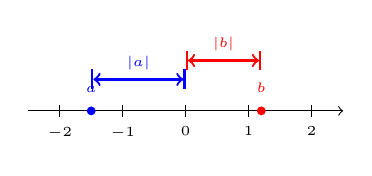
\begin{tikzpicture}[scale=0.8]
  % Number line
  \draw[->] (-2.5,0) -- (2.5,0);
  \foreach \x in {-2,-1,0,1,2} {
    \draw (\x,0.1) -- (\x,-0.1) node[below] {\tiny $\x$};
  }
  % Show |a| as distance
  \draw[thick, blue, |<->|] (-1.5,0.5) -- (0,0.5);
  \node[blue, above] at (-0.75,0.5) {\tiny $|a|$};
  \draw[thick, red, |<->|] (0,0.8) -- (1.2,0.8);
  \node[red, above] at (0.6,0.8) {\tiny $|b|$};
  % Points
  \fill[blue] (-1.5,0) circle (2pt) node[above=3pt] {\tiny $a$};
  \fill[red] (1.2,0) circle (2pt) node[above=3pt] {\tiny $b$};
\end{tikzpicture}
\caption{Absolute value as distance from zero on the number line.}
\end{marginfigure}

The set of rational numbers is defined as $\mathbb{Q} = \{ {p}/{q} \mid p, q \in \mathbb{Z}, q \neq 0 \}$, where ${p}/{q} = {r}/{s}$ if and only if $ps = qr$.\sidenote{This equivalence relation is crucial: $\frac{1}{2} = \frac{2}{4} = \frac{3}{6} = \cdots$ are all the same rational number. Formally, $\mathbb{Q}$ is constructed as a quotient set.} The integers are embedded in $\mathbb{Q}$ by identifying $n$ with ${n}/{1}$. In $\mathbb{Q}$, every non-zero element $x$ possesses a multiplicative inverse $x^{-1}$ such that $x \cdot x^{-1} = 1$.

This property distinguishes $\mathbb{Q}$ from $\mathbb{Z}$.

\dfn{Field}{A set $F$ is called a field if:
\begin{enumerate}[nolistsep, label=(\roman*)]
    \item $F$ is a commutative ring.
    \item For every $a \in F \setminus \{0\}$, there exists a multiplicative inverse $a^{-1} \in F$.
\end{enumerate}
In other words, a field is a structure where addition, subtraction, multiplication, and division (by non-zero divisors) are well-defined.}

Thus, $\mathbb{Q}$, $\mathbb{R}$, and $\mathbb{C}$ are fields, whereas $\mathbb{Z}$ is not. We call $\mathbb{Q}$ the field of quotients of $\mathbb{Z}$.\marginnote{Every integral domain can be embedded in its \emph{field of fractions} via the same construction used to build $\mathbb{Q}$ from $\mathbb{Z}$.}

The real numbers $\mathbb{R}$ may be constructed as the completion of $\mathbb{Q}$ (via Cauchy sequences or Dedekind cuts),\footnote{Richard Dedekind (1831--1916) introduced his ``cuts'' in 1872. A Dedekind cut partitions $\mathbb{Q}$ into two sets $A, B$ where every element of $A$ is less than every element of $B$. Each cut corresponds to a unique real number.} enabling the treatment of limits. The complex numbers $\mathbb{C} = \{ a + bi \mid a, b \in \mathbb{R} \}$ extend $\mathbb{R}$ to an algebraically closed field.\sidenote{A field is \emph{algebraically closed} if every non-constant polynomial has a root. The Fundamental Theorem of Algebra states that $\mathbb{C}$ has this property---every polynomial of degree $n$ has exactly $n$ roots (counted with multiplicity).} We recall Euler's formula, which connects the exponential function to trigonometry:
\[ e^{i\theta} = \cos \theta + i \sin \theta, \]
where $\theta$ is the argument of the complex number.

\begin{marginfigure}
\centering
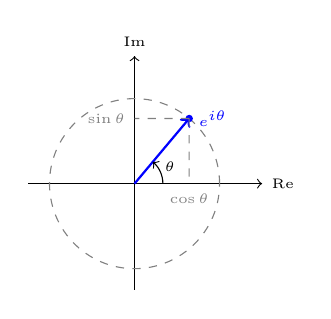
\begin{tikzpicture}[scale=0.9]
  % Axes
  \draw[->] (-1.5,0) -- (1.8,0) node[right] {\tiny Re};
  \draw[->] (0,-1.5) -- (0,1.8) node[above] {\tiny Im};
  % Unit circle
  \draw[dashed, gray] (0,0) circle (1.2cm);
  % Point on circle
  \coordinate (P) at (50:1.2);
  \draw[thick, blue, ->] (0,0) -- (P);
  \fill[blue] (P) circle (1.5pt);
  \node[blue, right] at (P) {\tiny $e^{i\theta}$};
  % Angle
  \draw[->] (0.4,0) arc (0:50:0.4);
  \node at (25:0.55) {\tiny $\theta$};
  % Projections
  \draw[dashed, gray] (P) -- ({1.2*cos(50)},0) node[below] {\tiny $\cos\theta$};
  \draw[dashed, gray] (P) -- (0,{1.2*sin(50)}) node[left] {\tiny $\sin\theta$};
\end{tikzpicture}
\caption{Euler's formula: $e^{i\theta}$ traces the unit circle in $\mathbb{C}$.}
\end{marginfigure}

Since $\mathbb{Q} \subset \mathbb{R} \subset \mathbb{C}$, we say that $\mathbb{R}$ is an \emph{extension field} of $\mathbb{Q}$, and $\mathbb{C}$ is an extension field of $\mathbb{R}$.

{\footnotesymbolstrue
\footnote{The study of field extensions forms the foundation of Galois theory, which connects group theory to the solvability of polynomial equations---one of the most beautiful bridges in mathematics.}
}
\end{document}
